%build with pdflatex to include frontpage

% This is the main report file

\documentclass{acm_proc_article-sp}
\usepackage[utf8]{inputenc}
\usepackage{listings}
\usepackage{pdfpages}
\begin{document}

\title{02321 Hardware/Software programming Jan 11}
\subtitle{[Technical University of Denmark]
%\titlenote{This report should also be available online at \texttt{www.retrospekt.dk/02228report}}
}

\numberofauthors{2}
\author{
\alignauthor 
Kim Rostgaard Christensen\\
       \email{s084283@student.dtu.dk}
\alignauthor 
Morten Hillebo (s072923)
       \email{s072923@student.dtu.dk}
}

%formal frontpage
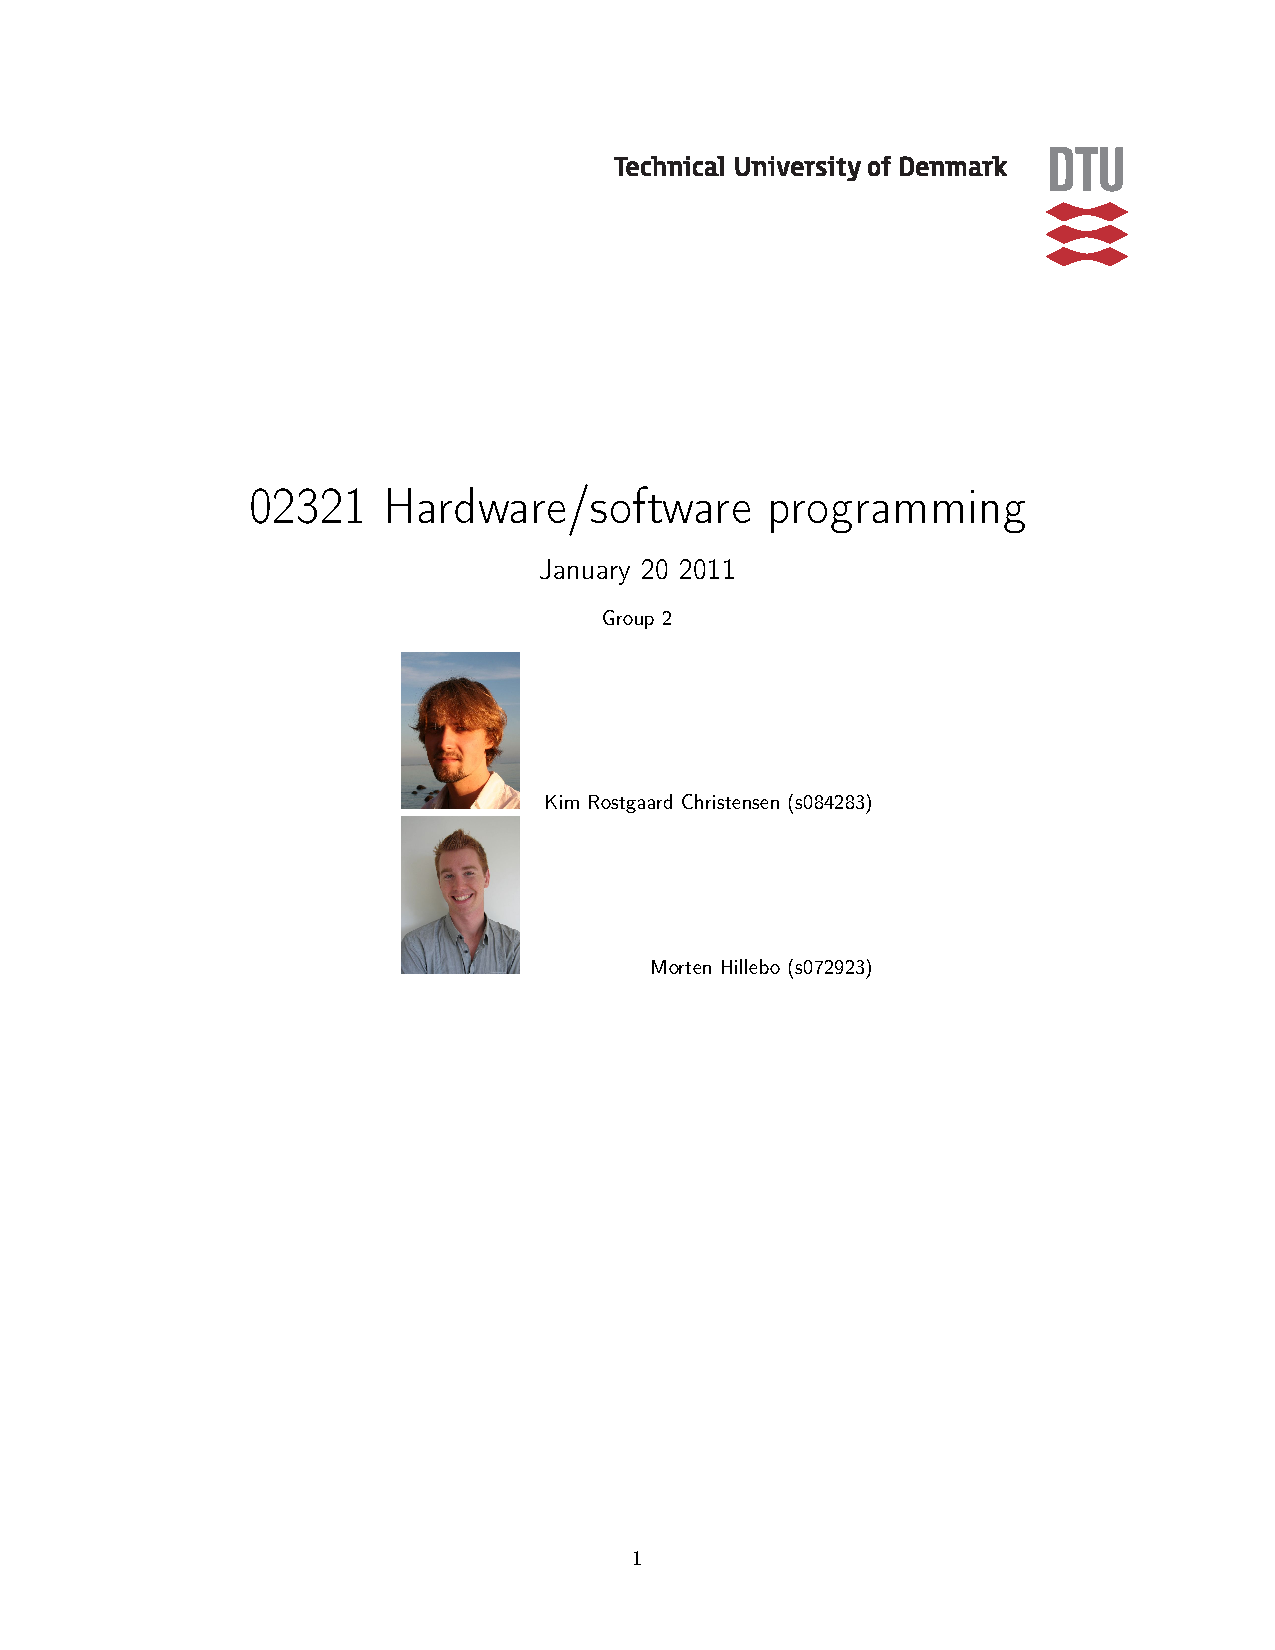
\includepdf{frontpage.pdf}

\maketitle

\begin{abstract}
%Abstract; A brief summary of all of the report including the conclusion section
%but excluding the acknowledgements, references and any appendixes.
This project will cover the implementations of the LC-3 computer and the classic video game Snake to a FPGA-board. 
The goal though out the project has been to implement all aspects of the computer and the video game on the FPGA-board so no help was needed by additional computer resources.
\end{abstract}

\section{Introduction}
\label{sec:introduction}

%TODO explain what the snake game is - briefly
The video snake game was first released in the mid 1970's and has since become a true video game classic. The game play involves navigating a snake looking thing around on the screen in search for food, that will make the snake gain body length and increment the game score. 
The walls and hurdles in the play area will cause the snake to die if they collide.
This project is about developing and implementing the snake game on the LC3 processor. 
%ACKNOWLEDGMENTS are optional
%\section{Acknowledgments}
%\input{acknowledgements.tex}
%Acknowledgments; Acknowledge any persons important to the work.

%References; A list of reference material used. All material must be cited in the
%text.
\section{Requirement specification}
The snake game requirement specification will be split in two sections, the minimal game implementation and the enhancements. 

\subsection{Minimal implementation}
The minimal implementation requirements was specified as below in arbitrary order.    
\begin{itemize}
\item Basic game logic (snake control, food consumption and growth)
\item Snake control via serial console 
\item Basic game display (level and snake by blocks) 
\item Simple levels
\end{itemize}

\subsection{Enhancements}
For the enhancements following improvement was specified also in arbitrary order.
\begin{itemize}
\item Control by the keyboard on the LC3 board 
\item Enhanced game display (sprites instead of blocks) 
\item Enhance game play various objects (power-ups)  
\item Complex levels with obstacles
\item Multi player functionality 
\end{itemize}

\section{Design}
There are many different options when it comes to the implementation of the game. The game can, for instance, run partially on a PC or completely on the LC3 - we have aimed for the latter.
\subsection{The game map}
For the game map a matrix, in the form of a two-dimensional array, is suitable. Every element of the map can be looked up by an x and y coordinate corresponding to their array indexes. The single element of the map is modelled as a tile that holds the value of this tile and other information which will be discussed later.

\subsection{Memory mapping}
In order to provide access from the programming language to the various I/O devices available, an interface is needed. This is in the form of a memory map, where certain areas of the memory is significant - or reserved. As the name would suggest, these memory areas are mapped onto the registers of the corresponding devices. A list of the I/O mappings can be found in table \ref{table:io_mappings} and \cite{patt2000introduction}

\begin{table}[h]
\centering
    \begin{tabular}{ | l | l | l |}
    \hline
     Register & Memory address \\ \hline 
    \hline
    Video memory           & xE000  \\ \hline
    Stdin Status Register  & xFE00  \\ \hline
    Stdin Data Register    & xFE02  \\ \hline
    Stdout Status Register & xFE04  \\ \hline
    Stdout Data Register   & xFE06  \\ \hline
    Switches Data Register & xFE0A  \\ \hline
    Buttons Data Register  & xFE0E  \\ \hline
    7SegDisplay Data Register  & xFE12  \\ \hline
    Leds Data Register  & xFE16  \\ \hline
    \end{tabular}
\caption{I/O mappings of the LC3}
\label{table:io_mappings}
\end{table}
Notice that the video memory is not a single address, but an address range up to the address before the stdin register.\\
The first design of the video memory used a classical write-only memory, but it became apparent when software was written that this was impractical in regards of house keeping. We realized that we could use the benefit of having complete control of the system to simply to software implementation. This became the birth of the hardware game model.
\subsubsection{Hardware game model}
The hardware game model is a somewhat lazy approach that takes advantage of the fact that the game is the only thing running on the computer.\\
It works by mapping the "content" of the tile to a memory location corresponding to the tile on the screen. It then changes from a value that has to be synced to video memory, to a pointer that has to have its value updated only once at every game update.\\\\
This of course requires that we must be able to also read from video memory. For this purpose, dual ported asynchronous ram\cite{chu2008fpga} is used for video memory. There is no complications with using asynchronous memory, as we only either read or write at one cycle. On the other hand, synchronous memory should also be safe to use, as a processor read operation takes two cycles, effectively putting the data on the bus in time for the value to be read during the second cycle. The only real difference is that the asynchronous memory uses one less register on the FPGA.

%Todo, drawing of the video memory

\subsection{Dynamic snake growth}
In order to keep track of the growth and location of the snake a clever design was found. For the snake, a linked list data structure would be used to keep track of the length and positions of the body elements. The update was now just a matter of going to the last element of the list and remove this.\\
Unfortunately, this design had one major flaw - no dynamic memory allocation is available on the LC-3. This is a show stopper as the linked list data structure requires a malloc call to be present on the system.\\
A different and more static approach was needed.
\subsection{(Static) Dynamic snake growth}
To emulate the behaviour of the linked list, every tile of the tilemap is equipped with a reference to the next element in a sequence, or null if no other element is linked to it. This takes up more memory (the size of a pointer multiplied by the number of elements in the map) but enables us to theoretically link every tile in the map to another tile.

\section{Discussion}

\subsection{Implementation issues}

\subsection{Hardware game model}
The use of the video ram for storing the hardware game model is a decision based on the fact that we are in complete control of the system, and no other processes or programs is run besides the game.\\\\
Video memory is usually synchronized from a software model, which our first implementation also was. Video memory a usually considered more volatile than system ram, as these belong to you once you have allocated it - at least on most operating systems.


\appendix

% The following two commands are all you need in the
% initial runs of your .tex file to
% produce the bibliography for the citations in your paper.
\bibliographystyle{plain}
%\nocite{*}
\bibliography{sigproc}  % sigproc.bib is the name of the Bibliography in this case
% You must have a proper ".bib" file
%  and remember to run:
% latex bibtex latex latex
% to resolve all references
%
% ACM needs 'a single self-contained file'!
%
%APPENDICES are optional
\section{Known bugs}
This section contains the bugs that we have identified, their severity and their status.
\subsection{Initial snake tail inconsistent}
When starting a new game, either at machine reset or when the snake dies, the tail follows an inconsistent linking leaving blank spaces for the first few game cycles. This is probably due to a bug in the way the snake body is generated in the "initialize\_snake" function.\\
The game works and renders fine after the first three cycles, and the bug does not affect gameplay.\\\\
Severity: Negligible\\
Status: Not fixed

\subsection{Snake stops on invalid button input}
When the user presses the btn5 or more than one button at once, the snake stops updating and the head becomes the tile rom index corresponding to the binary input on the buttons. The snake and the game continues if a valid button is pressed, but the graphics are incorrectly updated for the body elements.\\
This bug affects gameplay and is more severe as players often by accident press more than one button.\\\\
Severity: Important\\
Status: Not fixed

\section{Report distribution}
Kim Rostgaard Christensen
\begin{itemize}
\item stuff
\end{itemize}

Morten Hillebo
\begin{itemize}
\item stuff
\end{itemize}

%Appendixes; Appendixes holds, for example, results or figures that are not
%relevant to place in the body of the report. Appendixes should generally be
%avoided and might not be read by the course staff.


\end{document}
